\chapter{Revisão de literatura e conceituação teórica} \label{cap:conceitos}

Este capítulo tem como objetivo introduzir os conceitos teóricos básicos utilizados no documento e bases para apresentar a método.

\section{Problemas de Decisão} \label{sec:problemaDecisao}

Um problema $\Pi$ é dito um problema de decisão quando seu conjunto solução é composto apenas pelos elementos \textit{Sim} e \textit{Não}, ou seja:
\begin{equation} \label{eq:problemaDecisao}
\begin{split}
\Pi: D \rightarrow Im  \\
Im = \{ Sim, N\widetilde{a}o \}
\end{split}
\end{equation}

São exemplos de problemas de decisão:
\begin{itemize}
    \item Seja $x \in C$, sendo $x$ um número pertencente ao conjunto $C$, $x$ é o menor número deste conjunto?
    \item Seja um grafo $G(V,A)$ denotado pelos arestas $A$ e vértices $V$, existe um caminho do vértice $x$ para o vértice $y$ com custo menor que $c$?
\end{itemize}


\section{Problemas de Otimização} \label{sec:problemaOtimizacao}

Seja $\Pi$ um problema, S o conjunto de soluções viáveis para o mesmo e $f$ a função objetivo que associa uma solução $s_i$ a um valor numérico então temos:
\begin{equation}  \label{eq:problemaOtimizacao}
\begin{split}
S = \{s_1, s_2, \dots, s_n \} \\
f: S \rightarrow \mathbb{R}
\end{split}
\end{equation}

Um problema de otimização, em geral, pode ser de minimização ou de maximização.
$\Pi$ é um problema de minimização se ele consiste em determinar uma solução $s^*$ tal que:
\begin{equation}  \label{eq:problemaOtimizacaoMinimizar}
s^* \in S \mid f(s^*) \leq f(s), \forall s \in S
\end{equation}

De forma análoga um problema de minimização pode ser dado por:
\begin{equation}  \label{eq:problemaOtimizacaoMaximizar}
s^* \in S \mid f(s^*) \geq f(s), \forall s \in S
\end{equation}

Os problemas de otimização podem ser divididos em dois tipos:

\begin{itemize}
    \item Otimização contínua: nesse tipo de problema pelo menos uma das variáveis $x$ do conjunto de variáveis $X$ pode assumir infinitos valores;
    \item Otimização combinatória: problemas em que toda variável $x$ no conjunto de variáveis $X$ é discreta, podendo assumir apenas um número finito ou infinito porém contável de valores.
\end{itemize}

Desta forma, existe um número finito de soluções viáveis para um problema de otimização combinatória.
Para todo problema de decisão existe um problema de otimização associado, tomemos com exemplo os problemas da seção~\ref{sec:problemaDecisao} e teremos os seguintes problemas de otimização:

\begin{itemize}
    \item Seja um conjunto $C$, encontrar $x \in C \mid x < y, \forall y \in C$.
    \item Seja um grafo $G(V,A)$ denotado pelos arestas $A$ e vértices $V$, encontrar o menor caminho do vértice $x$ para o vértice $y$.
\end{itemize}

% \section{Problema do Mochileiro Viajante}\label{sec:ttp}

Adotemos a seguinte definição do PMV~\cite{Polyakovskiy:2014}. Dado um conjunto de cidades $ N = \{1, \dots, n\} $ e de distâncias $d_{ij}$ com $i, j \in N $ (indicando a distancia entre um par de cidades), o objetivo é visitar cada cidade exatamente uma vez sem repetições, iniciando da primeira até a última e então voltando para a primeira~\cite{Bonyadi:2013}.
Ademais, um conjunto possivelmente vazio de itens $ M_i = \{1, \dots, m_i\} $ está disponível para cada cidade $i$, cada item $k$ possui um lucro $p_{ik}$ e um peso $w_{ik}$ associados. Qualquer item pode ser coletado apenas na sua cidade até que a mochila esteja cheia (capacidade seja atendida ou o peso do item exceda a capacidade disponível), destarte o somatório de itens coletados está limitado a $W$, capacidade máxima da mochila (veículo).
Uma taxa de aluguel $R$ é paga por unidade de tempo gasta no percurso, sendo $v_{max}$ e $v_{min}$ a velocidade máxima e mínima, respectivamente, quando a mochila está cheia e vazia.

Denotemos então a rota selecionada por $x$ e sendo $y_{ik} \in \{0, 1\}$ uma variável binária igual a $1$ quando o item $k$ é coletado na cidade $i$, e $0$, caso contrário. Por último, denotemos $W_i$ o peso total da mochila no instante $i$ como o somatório do peso dos itens coletados ao sair da cidade $i$. Asism a função objetivo pode ser expressa pela Equação~\eqref{eq:fo}.
%
\begin{equation} \label{eq:fo}
\max f(x, y) = \sum\limits_{i=1}^n\sum\limits_{k = 1}^{m_i} p_{i,k}\;y_{i,k} - R
% \left(
% \frac{d_{x_n , x_1}}{v_{max} - vW_{x_n}} +
% \sum\limits_{i = 1}^{n - 1}\frac{d_{x_i , x_{i+1}}}{v_{max} - vW_{x_i}}
% \right)
\left(
\sum\limits_{i = 1}^{n - 1}\frac{d_{x_i , x_{i+1}}}{v_{max} - \nu W_{x_i}} +
\frac{d_{x_n , x_1}}{v_{max} - \nu W_{x_n}}
\right)
\end{equation}
% 
O objetivo é maximizar $f(x, y)$ dado que todas as cidades foram visitadas na rota $x$ (sem repetição) conforme Equação\ref{eq:repeatCity}, e sujeito a limitação da capacidade da mochila conforme Equação~\eqref{eq:capacity}, e a velocidade $\nu$ é dada pela Equação~\eqref{eq:currentSpeed}.
\begin{equation} \label{eq:repeatCity}
x_i = x_j \iff i = j, \forall x_i,x_j
\nu = \frac{v_{max} - v_{min}}{W}
\end{equation}

\noindent\begin{minipage}{.5\linewidth}
\begin{equation}\label{eq:capacity}
\sum\limits_{i=1}^n\sum\limits_{k = 1}^{m_i} w_{i,k}\;y_{i,k} \le W
\end{equation}

\end{minipage}
\noindent\begin{minipage}{.5\linewidth}
\begin{equation} \label{eq:currentSpeed}
\nu = \frac{v_{max} - v_{min}}{W}
\end{equation}
\end{minipage}

\subsection{Exemplo}\label{subsec:pmbExemplo}

Considere as cidade no mapa da Figura~\ref{fig:mapaItens}, existem 5 cidades e 4 itens. A cidade número 1 possui um item (de lucro 80, peso 4), cidade número 2 possui um item (lucro 50, peso 1), a cidade 3 não possui itens enquanto a cidade 4 possui 2 itens (lucro 100, peso 8 e lucro 10, peso 1).
Considerando uma velocidade mínima de 0,10, e máxima de 1,00, considere também uma mochila de capacidade 8 e uma taxa de aluguel 2,50.

\begin{figure}[htpb]
    \centering
    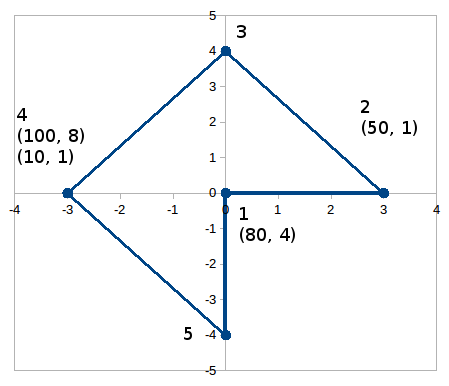
\includegraphics[width=0.6\linewidth]{figuras/pmv/mapaItens}
    \caption{Mapa de cidades e seus itens}
    \label{fig:mapaItens}
\end{figure}

Tomemos como exemplo a seguinte rota sem nenhum item coletado $x = \{ 1, 2, 3, 4, 5 \}$ logo $y = \{ 0, 0, 0, 0 \}$.
Para essa solução teremos o valor de função objetivo igual a -55,00.

Consideremos a gora a mesma rota coletando o item de maior lucro associado, então temos a rota $x = \{ 1, 2, 3, 4, 5 \}$, e a mochila $y = \{ 0, 0, 1, 0 \}$.
Agora teremos uma solução de valor -157,00.

Considerando ainda a mesma rota mas com dois itens coletados, temos a rota $x = \{ 1, 2, 3, 4, 5 \}$, e a mochila $y = \{ 0, 1, 0, 1 \}$.
Neste caso temos um valor de função objetivo igual a -4.70.


Nas Figuras~\ref{fig:pmvExemplo}, \ref{fig:pmvExemploAlterandoItens} e \ref{fig:pmvExemploAlterandoInicio} podemos ver a representação de soluções diferentes para a mesma instância de um PMV.
Cada apontador indica uma cidade sem itens a serem coletados, os presentes indicam itens a serem coletados com dois números associados ($p_i / w_i$, sendo $w_i$ e $p_i$ o peso e o lucro associados ao item $i$ respectivamente).
O stickman representa o início da rota, $W$ representa a capacidade de carga do veículo e $R$ a taxa de aluguel cobrada por unidade de tempo de uso do mesmo.

\begin{figure}[htpb]
    \centering
    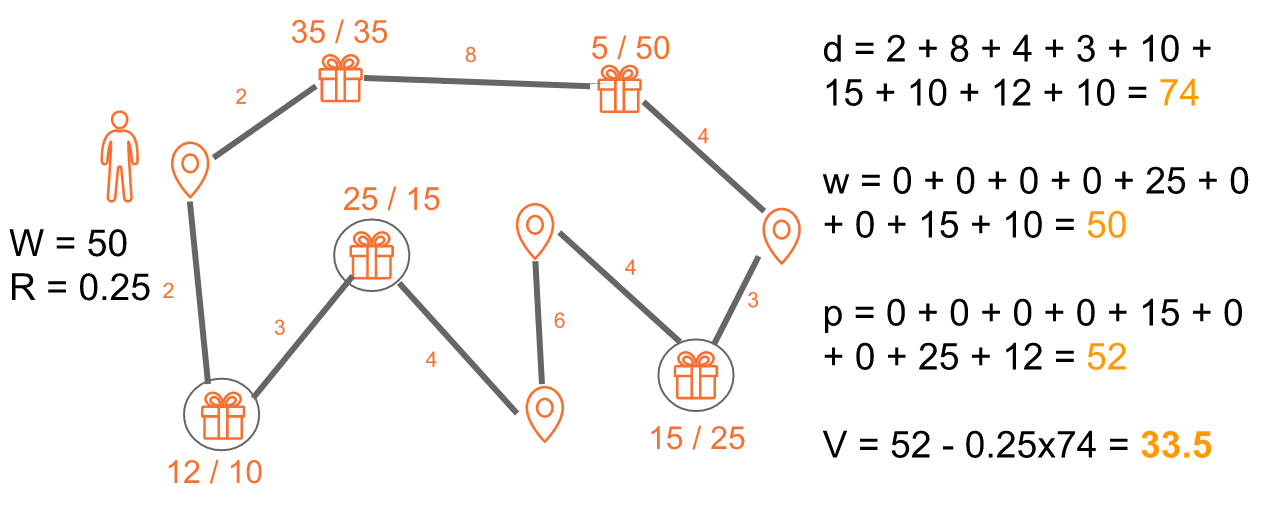
\includegraphics[width=0.8\linewidth]{figuras/pmv/example01.png}
    \caption{Exemplo de representação visual do PMV}
    \label{fig:pmvExemplo}
\end{figure}

Pelo primeiro exemplo, na Figura~\ref{fig:pmvExemplo}, vemos que são coletados 3 itens de valores 15, 25 e 12; e pesos de valor 25, 15, 10.
Desta forma temos um percurso total de distância 74, peso final do caminhão de 50, valor dos itens de 52.
Todos estes fatores aplicados à fórmula da função objetivo conferem um valor de solução de 33,5.

\begin{figure}[htpb]
    \centering
    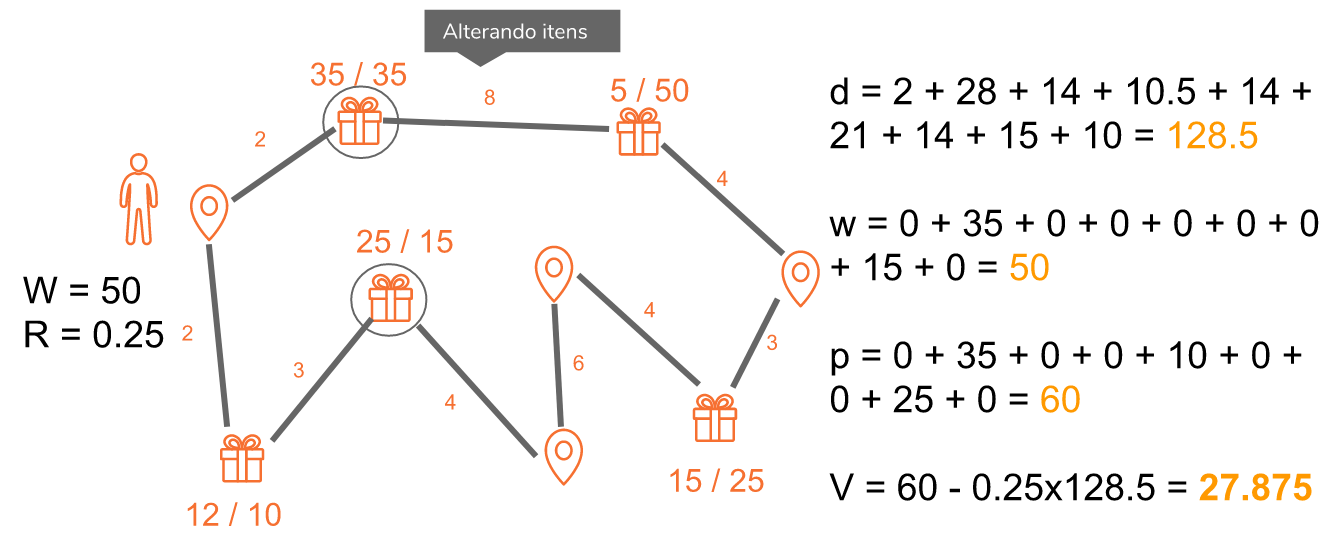
\includegraphics[width=0.8\linewidth]{figuras/pmv/example02.png}
    \caption{Mesmo conjunto de cidades e itens, alterando os itens coletados.}
    \label{fig:pmvExemploAlterandoItens}
\end{figure}

Mantendo a mesma rota do exemplo da Figura~\ref{fig:pmvExemplo} apenas alterando os itens coletados temos o exemplo da Figura~\ref{fig:pmvExemploAlterandoItens} que coleta apenas 2 itens de valores 35 e 25; além de pesos 35 e 15.
Neste caso se tem o mesmo peso final de 50 e um maior valor dos itens 60, contra 50 da solução anterior, porém coletar o item mais valioso e pesado logo no começo da rota prejudica todo o percurso fazendo com que sejam gastas muito mais unidades de tempo para percorrer todo o percurso, sendo um total de 128,5.
Logo temos um valor final de função objetivo de 27,875 que é menor que o anterior mesmo tendo coletado itens mais valiosos, isto ocorre porque apesar dos itens mais valiosos o custo pra coletá-los foi maior.

\begin{figure}[htpb]
    \centering
    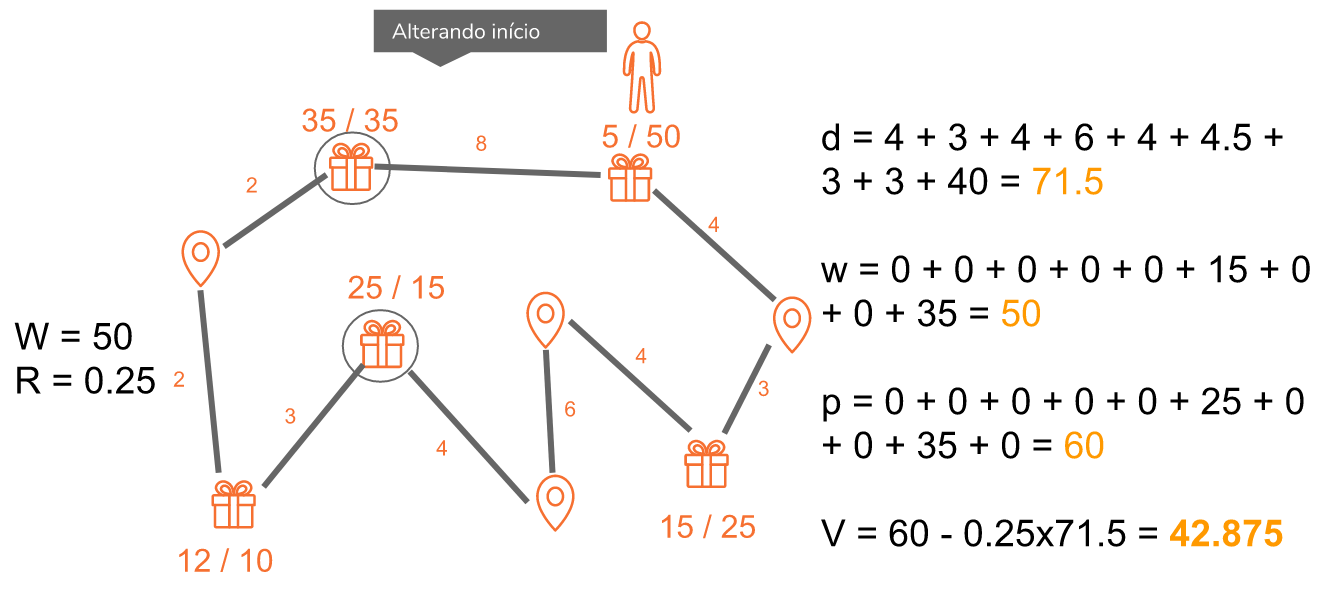
\includegraphics[width=0.8\linewidth]{figuras/pmv/example03.png}
    \caption{Mesmo conjunto de cidades e itens, alterando inicio da rota.}
    \label{fig:pmvExemploAlterandoInicio}
\end{figure}

No caso da Figura~\ref{fig:pmvExemploAlterandoInicio} foram mantidos os itens da Figura~\ref{fig:pmvExemploAlterandoItens} contudo foi trocada a cidade inicial do problema de forma que o veículo não precise transportar o item mais pesado por um período muito longo diminuindo assim o custo da rota para 71,5.
Não tendo alterado o os itens coletados o peso final e valor dos itens também se mantem constante, desta forma o novo valor de função objetivo é de 42,875 superando os valores encontrados nas duas soluções anteriores.

Mais alguns exemplos ilustrando o problema podem ser encontrados em \cite{Bonyadi:2013, Oliveira:2015}.


\section{Problema da Mínima Latência}\label{sec:mlp}

O Problema da Mínima Latência (PML) é um problema de otimização, sendo uma variante do PCV no qual o objetivo é minimizar o tempo de chegada (ou latência) aos vértices, e não a distância ou tempo da rota como no problema original.
O PML pode ser definido como um grafo direcionado $G=(V,E)$, onde $V=\{0,1,\dots,n\}$ é um conjunto de vértices e $E = \{(i, j) : i, j \in V, i \ne j \}$ um conjunto de arestas que conectam os vértices.
Para cada arco $(i,j)$ existe um tempo de viagem associado igual a $t(i,j)$. O vértice 0 representa o ponto de saída (depósito) e os demais os clientes a serem visitados.
O tempo de chegada (ou latência) a um cliente $i \in V$, é denotado por $l(i)$, o qual é definido pelo tempo de viagem do depósito até o vértice $i$.

\begin{figure}[htpb]
    \centering
    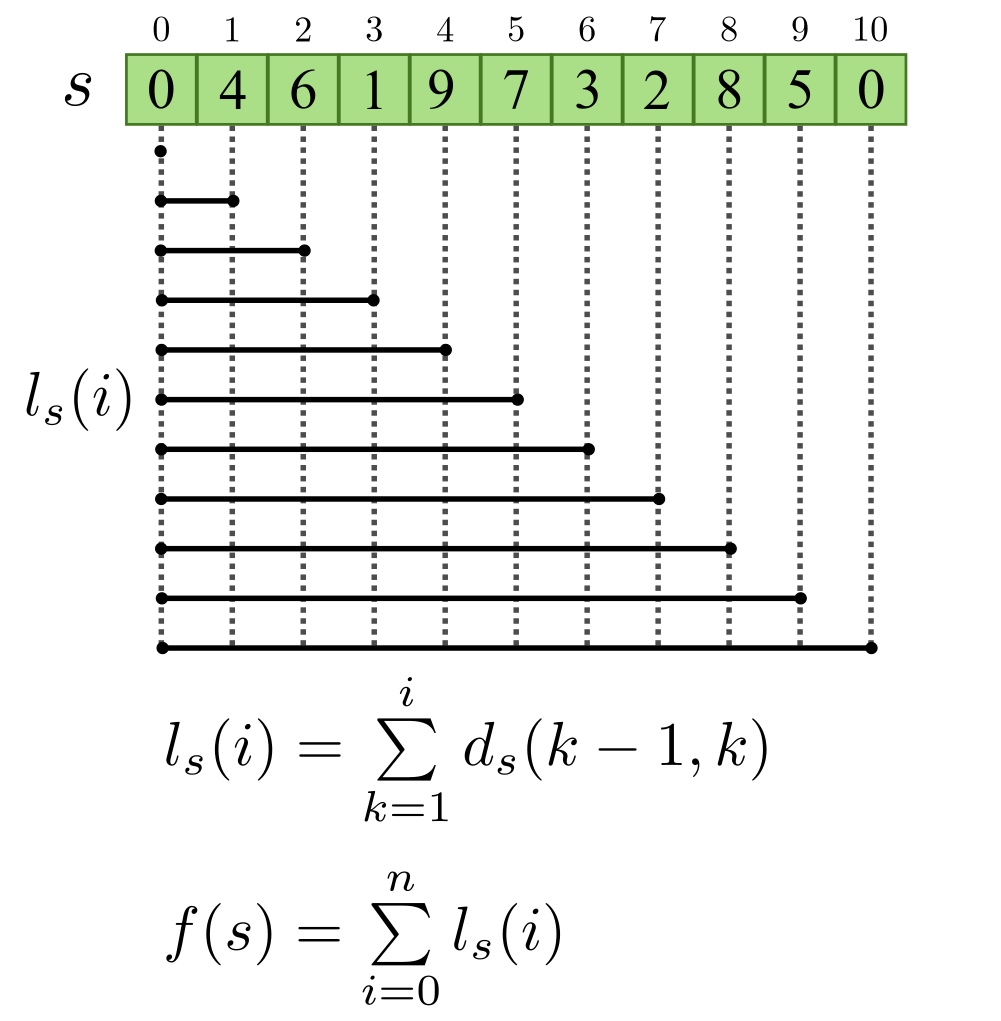
\includegraphics[width=0.6\linewidth]{figuras/pml/mlp}
    \caption{Exemplo de solução com as latências de cada cidade e cálculo da função objetivo}
    \label{fig:pmlDiagramaFormulas}
\end{figure}

O objetivo do PML é, iniciando do depósito, determinar o ciclo Hamiltoniano $s$ que minimize a latência expressa por $L(s)=\sum_{i=0}^{n} l(i)$ como pode ser visto na Figura~\ref{fig:pmlDiagramaFormulas}.
Assim sendo, uma solução viável do PML consiste numa permutação de $n$ clientes determinando a ordem de visita dos mesmos. Tomemos o exemplo a seguir, se $n=9$,  $s=[0,8,3,7,1,4,2,5,6,0]$ é uma solução viável para o PML (de fato, qualquer permutação $1..8$ começando e terminando no vértice zero é uma solução viável).

Apesar da formulação simples e de sua grande aplicação na otimização de latência em redes, o PML é um problema complexo, sendo provado que o PML é NP-Difícil~\cite{silva2012}. A despeito da semelhança na formulação do PML com a do Problema do Caixeiro Viajente (PCV) a sua função objetivo é mais complexa de ser calculada que a do PCV.
No PML, pequenas alterações no vetor solução podem levar a grandes alterações no resultado final da solução e a natureza não local da função objetivo faz com que uma simples inserção afete todas as latências subsequentes.
Na literatura, o PML também é conhecido Problema do Caixeiro Viajante Cumulativo \cite{bianco1993}, Problema do Entregador \cite{mladenovic2013} e Problema do Reparador Viajante. \cite{tsitsiklis1992}.

Em trabalhos recentes, um procedimento de busca local baseado em \emph{Graphics Processing Unit} (\emph{GPU}) e computação \emph{multi-core} foi proposto para o PML~\cite{wamca2016}.
A ideia foi chamada \emph{Distributed Variable Neighborhood Descent} (\emph{DVND}), tentando explorar diferentes estratégias de vizinhança simultaneamente para uma solução de entrada.

Em otimização, uma vizinhança é definida como um conjunto de operações chamados "movimentos", que são capazes de realizar pequenas alterações na solução de entrada.
Estas alterações podem ser, por exemplo, trocar dois elemento na permutação inicial, gerando dessa forma $\mathcal{O}(N^2)$ diferentes soluções (para o caso de uma permutação de tamanho $N$). Existe na literatura muitas dessas vizinhanças (como 2-Opt, OrOpt-1, OrOpt-2, Swap, ..., etc), conquanto por limitações computacionais estes são sempre explorados de forma sequencial, chamados de \emph{Variable Neighborhood Descent} (\emph{VND}).
Com o objetivo de encontrar um ótimo local para o PML, a ideia principal do DVND é usar GPU para obter operações de grão fino (que em geral são rápidas) e explorar toda a vizinhança $\mathcal{O}(N^2)$ mais rápido que em CPU (como explicado em~\cite{wamca2016}) e combinar as respostas das buscas, escolhendo a nova melhor solução.

\subsection{Exemplo}

% \begin{figure}[htpb]
%     \centering
%     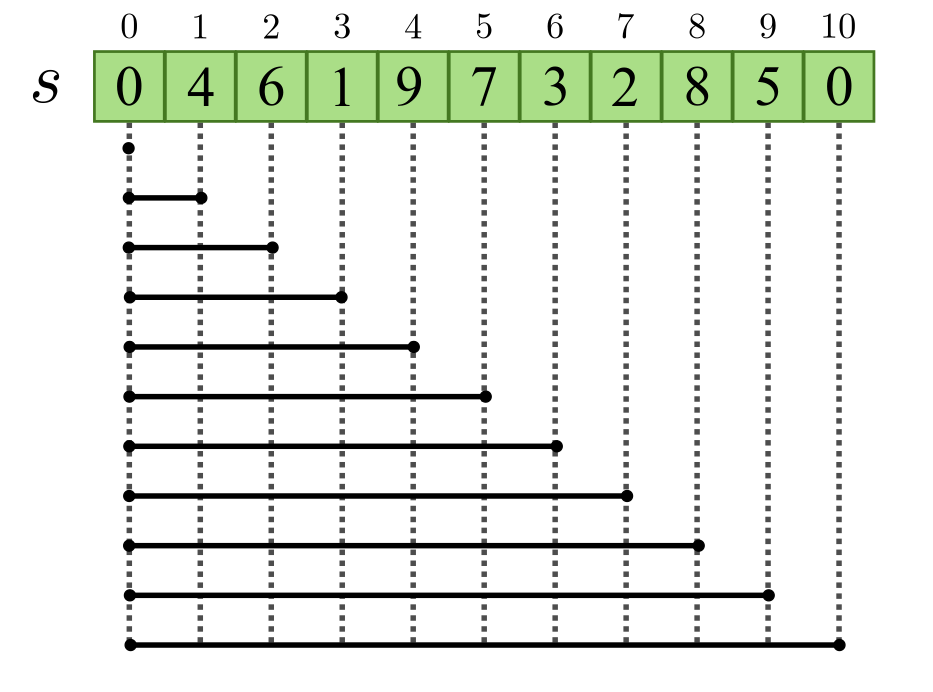
\includegraphics[width=0.6\linewidth]{figuras/pml/mlp-clean}
%     \caption{Exemplo de solução com as latências de cada cidade}
%     \label{fig:pml}
% \end{figure}

Pelo exemplo na Figura~\ref{fig:pmlDiagramaFormulas} podemos ver que o valor da latência $L(s)$ será dado palos somatórios das latências de todas as cidades, sendo $d_s^{i, j}$ a distância da cidade $i$ para a cidade $j$ na solução $s$, então temos:
$$ L(s) = \sum_{i=0}^n{l_s(i)} $$
$$ L(s) = l_s(0) + l_s(1) + l_s(2) + l_s(3) + l_s(4) + l_s(5) + l_s(6) + l_s(7) + l_s(8) + l_s(9) $$
$$ L(s) = 10d_s^{0, 4} + 9d_s^{4, 6} + 8d_s^{6, 1} + 7d_s^{1, 9} + 6d_s^{9, 7} + 5d_s^{7, 3} + 4d_s^{3, 2} + 3d_s^{2, 8} + 2d_s^{8, 5} + d_s^{5, 0}$$



\section{Busca local} \label{sec:buscaLocal}

\subsection{Vizinhança} \label{subsec:vizinhanca}

Seja $S$ o espaço de soluções de um problema de otimização $\Pi$, e $s \in S$ uma solução qualquer, considere a função objetivo $f: S \rightarrow \mathbb{R}$ que atribui um valor para cada solução.
Denotamos então por $N^x(s)$ o conjunto de soluções vizinhas de $s$ para a vizinhança $x$ com $N^x(s) \subset S$, em que as soluções dessa vizinhança podem ser obtidas de $s$ a partir da aplicação de determinadas operações.
Uma solução $s'$ é vizinha de $s$ (isto é $s' \in N^x(s)$) segundo uma vizinhança $s$ se $s'$ é alcançável a partir de $s$ fazendo uso de uma pequena perturbação nesta última.

\subsection{Movimento} \label{subsec:movimento}

% Seja $S$ o espaço de soluções de um problema de otimização $\Pi$, e $s \in S$ uma solução qualquer, considere a função objetivo $f: S \rightarrow \mathbb{R}$ que atribui um valor para cada solução.
Considere $m^x: S \rightarrow S$ a função que representa um movimento que leva uma solução $s$ a uma solução $s'$ ou de forma equivalente $s' = m^x \circ s$.
Designamos então o movimento $m^x \in M^x$ no conjunto de movimentos da vizinhança $x$.

Adicionalmente podemos definir o custo do movimento $m^x(s)$ em relação a solução $s$ como sendo a diferença entre o valor da solução $s'$ gerada ao aplicar este movimento à solução $s$ e o valor da solução $s$, conforme pode ser visto na Equação~\ref{eq:movimentoCusto}, iremos omitir a função $f$ e a vizinhança $x$ quando estiverem claros no contexto. Formalmente, a notação circunflexo representa a função $\widehat{m}: S \rightarrow \mathbb{R}$.
\begin{equation} \label{eq:movimentoCusto}
\widehat{m^x_f}(s) = f(s') - f(s)
\end{equation}

\subsubsection{Movimentos livres de contexto} \label{subsubsec:movimentosLivresDeContexto}

Um movimento $m$ é livre de contexto se ele sempre pode ser aplicado a uma solução $s$ sem gerar uma solução inválida.

\begin{equation} \label{eq:movimentoLivreDeContexto}
m \ \textrm{é livre de contexto} \  \iff m \circ s \in S, \forall s \in S
\end{equation}

Quando uma classe de movimentos é livre de contexto para um determinado problema então se pode dizer que a função a representar este movimento é fechada para o conjunto de soluções $S$.

A caracterização de um movimento como livre de contexto depende de suas restrições e da sua representação.
Desta forma, para o Problema do Caixeiro Viajante em que o grafo com as distâncias entre as cidades é completo, o movimento \textit{Swap} será livre de contexto contudo num grafo incompleto uma aplicação do \textit{Swap} pode gerar uma solução inviável pois pode não existir um determinado percurso após a alteração na solução.

\subsubsection{Movimentos parcialmente independentes} \label{subsubsec:movimentosParcialmenteIndependentes}

Movimentos parcialmente independentes são aqueles que podem ser aplicados simultaneamente a uma solução sem que o valor da solução obtida após a aplicação dos movimentos seja alterado, a independência parcial de movimentos pode ser definida para movimentos de vizinhanças diferentes.
Formalmente temos que dois movimentos $m_1$ e $m_2$ são parcialmente independentes se e somente se:
\begin{equation}
% \begin{align}
m_1 \textrm{ parcialmente independente } m_2 \iff f(m_1 \circ m_2 \circ s) = f(m_2 \circ m_1 \circ s) \label{eq:movimentosParcialmenteIndependentes}
% \end{align}
\end{equation}

\subsubsection{Movimentos independentes} \label{subsubsec:movimentosIndependentes}

Movimentos independentes são aqueles que a aplicação de um não altera o valor do outro, o valor do movimento $m_2$ aplicado à solução $m_1 \circ s$ é igual ao valor deste aplicado à solução $s$, a independência de movimentos pode ser definida para movimentos de vizinhanças diferentes.
Formalmente temos que dois movimentos $m_1$ e $m_2$ são independentes $m_1 \parallel m_2$ se e somente se:
\begin{equation}
% \begin{align}
m_1 \parallel m_2 \iff \widehat{m_1}(m_2 \circ s) = \widehat{m_2}(s) \land \widehat{m_2}(m_1 \circ s) = \widehat{m_1}(s)
% \end{align}
\end{equation}

\begin{theorem}%[Teorema da independência de movimentos]\label{teo:independenciaMovimentos}
Dois movimentos $m_1$ e $m_s$ são independentes então também são parcialmente independentes.
\begin{equation}
m_1 \parallel m_2 \implies m_1 \textrm{ parcialmente independente } m_2
\end{equation}

\begin{proof}
    Suponhamos que $m_1$ e $m_2$ sejam independentes mas não parcialmente independentes então $\widehat{m_1}(m_2 \circ s) = \widehat{m_2}(s) \land \widehat{m_2}(m_1 \circ s) = \widehat{m_1}(s)$ mas $f(m_1 \circ m_2 \circ s) \neq f(m_1 \circ m_1 \circ s)$
    \begin{align*}
        f(m_1 \circ m_2 \circ s) \neq & f(m_2 \circ m_1 \circ s) & \textrm{ De }(\ref{eq:movimentoCusto}) \\
        \widehat{m_1}(m_2 \circ s) + f(m_2 \circ s) \neq & \widehat{m_2}(m_1 \circ s) + f(m_1 \circ s) & \textrm{ De }\ (\ref{eq:movimentoCusto}) \\
        \widehat{m_1}(m_2 \circ s) + \widehat{m_2} + f(s) \neq & \widehat{m_2}(m_1 \circ s) + \widehat{m_1} + f(s) & \textrm{ Como } m_1 \parallel m_2 \\
        \widehat{m_1}(s) + \widehat{m_2} + f(s) \neq & \widehat{m_2}(s) + \widehat{m_1} + f(s) & \textrm{ Logo uma contradição } \bot
    \end{align*}
    
    Assim, por \textit{reductio ad absurdum}, temos que se $m_1$ e $m_2$ são independentes então também são parcialmente independentes.
\end{proof}
\end{theorem}

Outra propriedade interessante pode ser vista a seguir:
\begin{theorem}[Teorema da independência dos movimentos dois a dois]\label{teo:independenciaMovimentos2a2}
Se $m_1 \parallel m_2$ então o valor da solução gerada pela aplicação destes movimentos será igual ao valor anterior da solução somado ao valor dos movimentos.
\begin{equation}
\label{eq:movimentoCustoSomaDois}
m_1 \parallel m_2 \implies f(m_1 \circ m_2 \circ s) = \widehat{m_1}(s) + \widehat{m_2}(s) + f(s)
\end{equation}
\begin{proof}
    Suponhamos que $m_1$ e $m_2$ sejam independentes mas $f(m_1 \circ m_2 \circ s) \neq \widehat{m_1}(s) + \widehat{m_2}(s) + f(s)$.
    \begin{align*}
        f(m_1 \circ m_2 \circ s) \neq & \widehat{m_1}(s) + \widehat{m_2}(s) + f(s) & \textrm{ De } (\ref{eq:movimentoCusto}) \\
        \widehat{m_1}(m_2 \circ s) + f(m_2 \circ s) \neq & \widehat{m_1}(s) + \widehat{m_2}(s) + f(s) & \textrm{ De } (\ref{eq:movimentoCusto}) \\
        \widehat{m_1}(m_2 \circ s) + \widehat{m_2}(s) + f(s) \neq & \widehat{m_1}(s) + \widehat{m_2}(s) + f(s) & \textrm{ Como } m_1 \parallel m_2 \\
        \widehat{m_1}(s) + \widehat{m_2}(s) + f(s) \neq & \widehat{m_1}(s) + \widehat{m_2}(s) + f(s) & \textrm{ Logo uma contradição } \bot
    \end{align*}
    
    Assim, por \textit{reductio ad absurdum}, temos que se $m_1$ e $m_2$ são independentes então $f(m_1 \circ m_2 \circ s) = \widehat{m_1}(s) + \widehat{m_2}(s) + f(s)$.
\end{proof}
\end{theorem}

\subsubsection{Movimentos estritamente independentes} \label{subsubsec:movimentosEstritamenteIndependentes}

Dois movimentos $m_1$ e $m_2$ são estritamente independentes quando são independentes e podem ser aplicados simultaneamente a uma solução sem que a alteração feita por um gere algum conflito na causada pelo outro, a independência de movimentos pode ser definida para movimentos de vizinhanças diferentes.
Formalmente temos que dois movimentos $m_1$ e $m_2$ são estritamente independentes $m_1 \parallel_e m_2$ se e somente se:
\begin{equation}  \label{eq:movimentosIndependentes}
m_1 \parallel_e m_2 \iff m_1(m_2(s)) = m_2(m_1(s)) = m_1 \circ m_2 \circ s = m_2 \circ m_1 \circ s
\end{equation}

Pela Equação~\ref{eq:movimentosParcialmenteIndependentes} e pela definição de custo do movimento (Equação~\ref{eq:movimentoCusto}) podemos ver que um movimento estritamente independente também será um movimento independente.

A mesma ideia pode ser aplicada para um conjunto de movimentos $M = \{ m_1, m_2, m_3, ...\}$, são ditos estritamente independentes se para uma solução $s$ qualquer e para todo subconjunto não-vazio $M' = \{ m_1, m_2, m_3, \dots, m_k \} \subseteq M$ temos $m_1 \circ m_2 \circ m_3 \circ ...\circ m_k \circ s = m_2 \circ m_1 \circ m_3 \circ ...\circ m_k \circ s$ para qualquer permutação dos movimentos em $M'$.
% $\widehat{m_1}(s) + \widehat{m_2}(s) + \widehat{m_3}(s) + \dots + \widehat{m_k}(s) = \widehat{m_1}(m_2 \circ m_3 \circ ...\circ m_k \circ s)$. 

Pela Equação~\ref{eq:movimentosIndependentes} pode-se perceber que movimentos estritamente independentes são operações comutativas, pela própria definição.


Assim podemos estender a definição da vizinhança $x$ para:
\begin{equation}  \label{eq:vizinhanca}
N(s) = \{ m_i \circ s \mid \forall m_i \in M \}
\end{equation}

Cabe aqui destacar que a independência de movimentos é uma relação dada dois a dois entre os movimentos, logo não existe transitividade na relação de independência de destes, ou seja, se temos dois movimentos independentes $m_1 \parallel m_2$ e outro movimento $m_3$ tal que $m_3 \parallel m_2$ então \textbf{não} implica que $m_1 \parallel m_3$.
Pode existir um conflito, logo os movimentos $m_1 \nparallel m_3$ ou seja, seriam conflitantes.
Assim em termos de conflitos entre movimentos podemos escrever:
\begin{equation}
m_1 \parallel m_2 \land m_2 \parallel m_3 \centernot\implies m_1 \parallel m_3
\end{equation}

Tenhamos como exemplo o caso a seguir para a vizinhança de Swap, sendo eles $Swap(2,3), Swap(3,6), Swap(4,5)$, neste caso podemos ver que $Swap(2,3) \parallel Swap(4,5)$ e que $Swap(4,5) \parallel Swap(3,6)$ contudo $Swap(2,3) \nparallel Swap(3,6)$.

Para fins dessa dissertação, por questão de simplificação de notação, deste ponto em diante as referências a \textit{movimentos independentes} estão referenciando \textit{movimentos estritamente independentes}.

% Estou achadno a prova do teorema muito fraca
% % Igor coloquei isso aqui como um Teorema, não sei se é muito ambicioso da minha parte
% 
\begin{theorem}[Teorema da independência de movimentos]\label{teo:independenciaMovimentos}
Seja um conjunto $M'$ com movimentos livres de contexto em que todos os movimentos são independentes entre si dois a dois, ou seja $m_i \parallel m_j \mid \forall m_i, m_j \in M'$, com $m_i \ne m_j$.
E seja $s'$ a solução dada pela aplicação de todos os movimentos à solução inicial $s$, logo o valor da solução resultante $s'$ será dado pelo somatório do valor de cada movimento. Assim, pode-se escrever:

% \begin{align*} \label{eq:teo:independenciaMovimentos}
% m_1 \parallel m_2 \implies& s' = m_1 \circ m_2 \circ s \\
% m_1 \parallel m_2 \implies& f(s') = \widehat{m_1}(s) + \widehat{m_2}(s) + f(s) \\
% \end{align*}

% \begin{align*}
\begin{equation}
    \label{eq:teo:independenciaMovimentos}
    \begin{split}
        m_i \parallel m_j, \forall m_i, m_j \in M' \implies& s' = m_1 \circ m_2 \circ \dots \circ m_n \circ s \\
        m_i \parallel m_j, \forall m_i, m_j \in M' \implies& f(s') = f(s) + \widehat{m_1}(s) + \widehat{m_2}(s)+ \widehat{m_3}(s) + \dots + \widehat{m_n}(s) \\
        m_i \parallel m_j, \forall m_i, m_j \in M' \implies& f(s') = f(s) + \sum_i^n{\widehat{m_i}(s)}
    \end{split}
\end{equation}
% \end{align*}
\end{theorem}

\begin{proof}\label{proof:independenciaMovimentos}
% ---
% Prova por contradição
% ---
Suponhamos um conjunto $M = \{ m_1, m_2, \dots, m_n \}$ com $n$ movimentos independentes dois a dois mas $f(m_1 \circ m_2 \circ \dots \circ m_n \circ s) \neq f(s) + \widehat{m_1}(s) + \widehat{m_2}(s)+ \widehat{m_3}(s) + \dots + \widehat{m_n}(s)$.

\begin{align*}
    f(m_1 \circ m_2 \circ \dots \circ m_n \circ s) \neq f(s) + \widehat{m_1}(s) + \widehat{m_2}(s) + \dots + \widehat{m_n}(s) & \\
    \widehat{m_1}(m_2 \circ \dots \circ m_n \circ s) + f(m_2 \circ \dots \circ m_n \circ s) \neq f(s) + \widehat{m_1}(s) + \widehat{m_2}(s) + \dots + \widehat{m_n}(s) & \ [1] \\
    \widehat{m_1}(s) + f(m_2 \circ \dots \circ m_n \circ s) \neq f(s) + \widehat{m_1}(s) + \widehat{m_2}(s) + \dots + \widehat{m_n}(s) & \\
    \widehat{m_1}(s) + \widehat{m_2}(m_3 \circ \dots \circ m_n \circ s) + f(m_3 \circ \dots \circ m_n \circ s) \neq f(s) + \widehat{m_1}(s) + \widehat{m_2}(s) + \dots + \widehat{m_n}(s) & \ [2] \\
    \widehat{m_1}(s) + \widehat{m_2}(s) + f(m_3 \circ \dots \circ m_n \circ s) \neq f(s) + \widehat{m_1}(s) + \widehat{m_2}(s) + \dots + \widehat{m_n}(s) & \\
    \vdots & \\
    \widehat{m_1}(s) + \widehat{m_2}(s) + \dots + \widehat{m_n}(s) + f(s) \neq f(s) + \widehat{m_1}(s) + \widehat{m_2}(s) + \dots + \widehat{m_n}(s) & \ [3] \\
\end{align*}

Os passos acima se dão conforme:
\begin{align*}
[1] \ & m_1 \parallel m_i \mid \forall m_i \in M \\
[2] \ & m_2 \parallel m_i \mid \forall m_i \in M \\
[3] \ & \textrm{Logo temos uma contradição} \bot
\end{align*}

Desta forma, por \textit{reductio ad absurdum} demonstramos que se os movimentos são independentes então o valor da solução resultante se dará pelo somatório da solução anterior com o valor dos movimentos.

% ---
% Indução
% ---
% Pela Equação~\ref{eq:movimentoCustoSomaDois} temos que $f(m_1 \circ m_2 \circ s) = \widehat{m_1}(s) + \widehat{m_2}(s) + f(s)$, supondo por hipótese de indução que $f(m_1 \circ m_2 \circ \dots \circ m_n \circ s) = f(s) + \widehat{m_1}(s) + \widehat{m_2}(s) + \dots + \widehat{m_n}(s)$

% \begin{align*}
%     f(m_1 \circ m_2 \circ \dots \circ m_n \circ m_{n+1} \circ s) = & f(m_{n+1} \circ m_1 \circ m_2 \circ \dots \circ m_n \circ s) \\
%     f(m_1 \circ m_2 \circ \dots \circ m_n \circ m_{n+1} \circ s) = & \widehat{m_{n+1}}(m_1 \circ m_2 \circ \dots \circ m_n \circ s) + f(m_1 \circ m_2 \circ \dots \circ m_n \circ s) \\
% \end{align*}

% % \widehat{m_1}(s) + \widehat{m_2}(s) + \dots + \widehat{m_n}(s) + f(s)
% Fazendo $s_2 = m_2 \circ \dots \circ m_n \circ s$.
% \begin{align*}
%     f(m_1 \circ m_2 \circ \dots \circ m_n \circ m_{n+1} \circ s) = & \widehat{m_{n+1}}(m_1 s_2) + f(m_1 \circ m_2 \circ \dots \circ m_n \circ s) \\
%     f(m_1 \circ m_2 \circ \dots \circ m_n \circ m_{n+1} \circ s) = & \widehat{m_{n+1}}(s_2) + f(m_1 \circ m_2 \circ \dots \circ m_n \circ s)
% \end{align*}

% Pois $m_{n+1} \parallel m_1$, fazendo agora $s_3 = m_3 \circ \dots \circ m_n \circ s$.
% \begin{align*}
%     f(m_1 \circ m_2 \circ \dots \circ m_n \circ m_{n+1} \circ s) = & \widehat{m_{n+1}}(m_2 \circ \dots \circ m_n \circ s) + f(m_1 \circ m_2 \circ \dots \circ m_n \circ s)\\
%     f(m_1 \circ m_2 \circ \dots \circ m_n \circ m_{n+1} \circ s) = & \widehat{m_{n+1}}(m_2 \circ s_3) + f(m_1 \circ m_2 \circ \dots \circ m_n \circ s)\\
%     f(m_1 \circ m_2 \circ \dots \circ m_n \circ m_{n+1} \circ s) = & \widehat{m_{n+1}}(s_3) + f(m_1 \circ m_2 \circ \dots \circ m_n \circ s)\\
%     \vdots \\
%     f(m_1 \circ m_2 \circ \dots \circ m_n \circ m_{n+1} \circ s) = & \widehat{m_{n+1}}(s) + f(m_1 \circ m_2 \circ \dots \circ m_n \circ s)\\
%     f(m_1 \circ m_2 \circ \dots \circ m_n \circ m_{n+1} \circ s) = & \widehat{m_{n+1}}(s) + \widehat{m_1}(s) + \widehat{m_2}(s) + \dots + \widehat{m_n}(s) + f(s)
% \end{align*}

% Logo, por indução finita temos que $m_i \parallel m_j, \forall m_i, m_j \in M' \implies f(s') = f(s) + \sum_i^n{\widehat{m_i}(s)}$.

\end{proof}


\subsection{First Improvement vs Best Improvement} \label{subsec:firstBestImprovement}

As estratégias \textit{First Improvement} (Primeira melhora) e \textit{Best Improvement} (Melhor melhora) recebem como parâmetro a solução da iteração corrente para gerar seus vizinhos e escolhem uma solução a ser retornada conforme um critério específico, a saber, a primeira solução a melhorar a atual e a melhor solução encontrada na vizinhança, respectivamente.

\begin{algorithm}[htpb]
\caption{First Improvement para um problema de minimização}
\label{alg:firstImprovement}
\begin{algorithmic}[1]
    \Function{FirstImprovement}{Solução: $s$, Operador de vizinhança: $x$}
        % \For{$s' \in N^x(s)$} \Comment{Para cada solução $s'$ vizinha de $s$}
        %     \If{$f(s') < f(s)$} \Comment{Se a solução for melhor que a atual}
        %         \Return{$s'$}
        %     \EndIf
        % \EndFor
        \For{$m_i \in M$} \Comment{Para cada movimento $m_i \in M$}
            \If{$\widehat{m_i}(s) < 0$} \Comment{Se a solução for melhor que a atual}
                \Return{$m_i \circ s$}
            \EndIf
        \EndFor
        \Return{$s$} \Comment{Caso não consiga melhorar retorna a própria solução}
    \EndFunction
\end{algorithmic}
\end{algorithm}

Podemos ver o pseudocódigo do \textit{First Improvement} no Algoritmo~\ref{alg:firstImprovement} que consiste de enumerar os vizinhos até encontrar o primeiro que seja melhor que a solução atual, este então é retornado como resposta do método.
O método de \textit{Best Improvement} (Algoritmo~\ref{alg:bestImprovement}) consiste em enumerar toda a vizinhança guardando a informação do melhor encontrado até o momento, e então retornar o melhor resultado encontrado.

\begin{algorithm}[htpb]
\caption{Best Improvement para um problema de minimização}
\label{alg:bestImprovement}
\begin{algorithmic}[1]
    \Function{BestImprovement}{Solução: $s$, Operador de vizinhança: $x$}
        % \Let{$s^{best}$}{$s$} \Comment{Melhor solução encontrada}
        % \For{$s' \in N^x(s)$} \Comment{Para cada solução $s'$ vizinha de $s$}
        %     \If{$f(s') < f(s)$} \Comment{Se a solução for melhor que a atual altera a melhor solução encontrada}
        %         \Let{$s^{best}$}{$s'$}
        %     \EndIf
        % \EndFor
        \Let{$s^{best}$}{$s$} \Comment{Melhor solução encontrada}
        \For{$m_i \in M$} \Comment{Para cada movimento $m_i \in M$}
            \If{$\widehat{m_i}(s) < f(s^{best}) - f(s)$} \Comment{Se a solução for melhor que a atual altera a melhor solução encontrada}
                \Let{$s^{best}$}{$m_i \circ s$}
            \EndIf
        \EndFor
        \Return{$s^{best}$} \Comment{Retorna a melhor solução encontrada}
    \EndFunction
\end{algorithmic}
\end{algorithm}

O \textit{First Improvement} pode ser uma opção ao método de \textit{Best Improvement} quando a enumeração de toda a vizinhança é uma atividade muito custosa.
% Posso afirmar isso?
Embora não haja um paralelo para a definição matemática formal da solução $s'$ retornada pelo \textit{First Improvement} esta pode ser definida para o \textit{Best Improvement} de maneira simples por $s' \in N^x(s) \mid f(s') < f(s), \forall s \in N^x(s)$, o que, como veremos a seguir na seção~\ref{sec:otimoLocalGlobal}, corresponde ao ótimo local para a solução $s$ segundo a vizinhança $x$.
Em termos de movimento temos $s' = m' \circ$ com $\widehat{m'}(s) < \widehat{m_i}(s) \mid \forall m_i \in M$.

\subsection{Random Selection}

Nesta estratégia \textit{Random Selection} (Escolha Aleatória) é selecionada uma solução aleatoriamente entre aquelas que melhoram a solução atual.

\begin{algorithm}[htpb]
\caption{Random Selection para um problema de minimização}
\label{alg:randomSelection}
\begin{algorithmic}[1]
    \Function{RandomSelection}{Solução: $s$, Operador de vizinhança: $x$}
        \Let{$S_{imp}$}{$\emptyset$} \Comment{Conjunto com soluções de melhora}
        \For{$m_i \in M$} \Comment{Para cada movimento $m_i \in M$}
            \If{$\widehat{m_i}(s) < 0$} \Comment{Se a solução for melhor que a atual}
                \Let{$S_{imp}$}{$S_{imp} \cup \{ m_i \circ s\}$} \label{alg:randomSelection:salvaMelhora} \Comment{Adiciona ao conjunto de soluções de melhora}
            \EndIf
        \EndFor
        \Return{$Any(S_{imp})$} \Comment{Retorna uma das soluções de melhora}
    \EndFunction
\end{algorithmic}
\end{algorithm}

A estratégia \textit{Random Selection} (mostrada no Algoritmo~\ref{alg:randomSelection}) navega pelas soluções e na mantém as melhores soluções que melhoram a solução atual, conforme linha~\ref{alg:randomSelection:salvaMelhora}, para ao final retornam uma deste grupo.

\subsection{Multi Improvement}

Uma alternativa ao \emph{Best Improvement}, \emph{First Improvement} e ao \emph{Random Selection} é o \emph{Multi Improvement}~\cite{rios2015}.
A ideia é combinar um conjunto de movimentos independentes e executá-los simultaneamente sobre a solução de entrada.
Note que, embora consista na aplicação de diversos movimentos, somente uma única solução vizinha é gerada.
O \emph{Multi Improvement} pode ser utilizado em qualquer contexto que o \emph{Best Improvement} ou \emph{First Improvement} se encaixe (etapa de Exploração de Vizinhança ou {\it Neighborhood Exploration}), porém caso só exista um único movimento independente na vizinhança, ele terá comportamento equivalente ao Best Improvement.
Assim a solução $s'$ retornada por uma iteração do \emph{Multi Improvement} após ser aplicado a uma solução $s$ é dada por $s' = m_1 \circ m_2 \circ \dots m_k \circ s$ com os movimentos independentes $\{ m_1, m_2, \dots, m_k \} \subset M$.

O \emph{Multi Improvement} se encaixa particularmente bem com o conceito de \emph{SIMD} (\emph{Single Instruction Multiple Data}), presente nas GPUs, sendo sua complexidade similar ao \emph{Best Improvement} (todos movimentos da vizinhança são enumerados), seguido de uma etapa de junção (ou {\it merge}) dos movimentos independentes.
Podem existir cenários em que o \emph{Best Improvement} seja mais eficiente (com poucos movimentos independentes), embora já tenha sido demonstrado na literatura que mesmo casos com apenas dois movimentos independentes acabam mais promissores no \emph{Multi Improvement} do que no \emph{Best Improvement}. % Não seria importante colocar a referência disso?

\subsection{Passo iterativo} \label{subsec:passoIterativo}
% Posso fazer essa definição que estou fazendo aqui?
% Pensei em fazer isso para facilitar explicar algumas coisas mais pra frente

Em geral, um algoritmo de busca local é um processo iterativo pesado que tem como objetivo encontrar uma solução melhor que a atual dentro de um espaço de busca.
A solução recebida como entrada pode ser aleatória ou advinda de alguma heurística construtiva, a intenção do processo é aprimorar o resultado encontrado.

Cada iteração da busca local tenta encontrar a melhor solução mediante alguma alteração na solução atual, então o processo se repete na solução gerada até que nenhuma melhora seja possível.

\begin{algorithm}[htpb]
\caption{Busca local definida de forma genérica}
\label{alg:localSearch}
\begin{algorithmic}[1]
    \Function{LocalSearch}{Solução: $s$}
        \While{$f(Alterar(s)) < f(s)$} \Comment{Cada iteração corresponde a um passo iterativo da busca local}
            \Let{s}{$Alterar(s)$}
        \EndWhile
        \Return{$s$} \Comment{Retorna a melhor solução encontrada}
    \EndFunction
\end{algorithmic}
\end{algorithm}

Supondo que $Alterar(s)$ (apresentado do Algoritmo~\ref{alg:localSearch}) retorna uma solução melhor que a atual segundo alguma alteração, convencionemos então chamar de \textbf{passo iterativo} cada iteração da busca local em que o processo obtém uma solução melhor que a atual e salva o melhor resultado encontrado até o momento.
Assim para uma solução $s$ o passo iterativo é dado pela Equação~\ref{eq:passoIterativo}.

\begin{equation} \label{eq:passoIterativo}
\rho(s) = min(s, Alterar(s)) \implies f(\rho(s)) \le f(s)
\end{equation}


\section{Ótimo global vs Ótimo local} \label{sec:otimoLocalGlobal}

O ótimo global e ótimo local são exemplificados na Figura~\ref{fig:espacoDeBusca}.
Uma solução $s^* \in S$ é dita \textbf{ótimo global} para um problema $\Pi$ quando não existe outra solução viável $s'$ com melhor valor de função objetivo, formalmente temos que $s^*$ é ótimo global quando:
\begin{itemize}
    \item $\forall s' \in S \mid f(s') \le f(s^*), s' \neq s^* $ para um problema de maximização;
    \item $\forall s' \in S \mid f(s') \ge f(s^*), s' \neq s^* $ para um problema de minimização.
\end{itemize}

Considere uma busca local de \textit{Best Improvement} $H$ para o problema $\Pi$ sobre a estrutura de vizinhança $N^x$, após aplicar $H$ a uma solução inicial $s^0 \in S$ é obtido um conjunto de soluções $N^x(s^0)$ vizinhas, assim o \textbf{ótimo local} (\textit{mínimo local}) segundo a vizinhança $N^x$ para a solução $s^0$ é dado por:
\begin{itemize}
    \item $s'' \in N^x(s^0) \mid f(s'') < f(s'), \forall s' \in N^x(s^0), s'' \neq s'$, para um problema de minimização;
    \item $s'' \in N^x(s^0) \mid f(s'') > f(s'), \forall s' \in N^x(s^0), s'' \neq s'$, para um problema de maximização.
\end{itemize}

Em linhas gerais um \textbf{ótimo local} é a solução com melhor valor de função objetivo para um contexto local, seja uma vizinhança ou o conjunto imagem de uma heurística.


% \section{Classes de Problemas} \label{sec:classesProblemas}

\section{Meta-heurísticas} \label{sec:metaHeuristicas}

Uma meta-heurísticas diferencia-se de uma heurística por não ser acoplada a um problema específico ou classe de problemas.
Meta-heurísticas fazem uso de artifícios capazes de encontrar soluções e aprimorar as já encontradas enquanto procuram escapar de mínimos locais.
Na literatura são utilizadas em trabalhos que tratam de problemas da classe NP-Difícil devido a simplicidade de implementação e a intratabilidade da solução exata de tais problemas.
Assim, esses algoritmos são ferramentas robustas para serem aplicadas na resolução prática de problemas de otimização combinatória, sendo uma alternativa quando o respectivo algoritmo exato não é conhecido ou exige um alto tempo de execução \cite{glover2006handbook}.

As meta-heurísticas evoluem iterativamente conforme a parametrização fornecida até atingir um \textbf{Critério de Parada}, que pode também estar sujeito aos parâmetros do método.
O critério de parada, em geral, está associado ao número de iterações, tempo de execução, um parâmetro de qualidade ou número de iterações sem melhora.

% \section{Heurísticas} \label{sec:heuristicas}

\section{Dataflow} \label{sec:conceitosDataflow}
% Essa parte tá bem próxima da tese do Marzulo

Atualmente os processadores no mercado de computadores seguem, em geral, o modelo de \textit{Von Neumann}.
No referido modelo, a execução das instruções é guiada por um fluxo de controle, ou seja, segundo a ordem que aparecem no programa, desta forma se faz necessário um \textit{Program Counter} (Contador de Programa) para indicar qual a próxima instrução a ser executada.
O contador também pode ser alterado por instruções de desvio, e laços de repetição ou qualquer tipo de comando de execução condicional.

Note que este modelo é intrinsecamente sequencial. No entanto, tenta-se resgatar paralelismo em nível de instruções com técnicas como pipelining~\cite{patterson2003computerOrganization}, predição de desvio~\cite{patterson2003computerOrganization} e renomeamento de registradores~\cite{patterson2012}.

O modelo dataflow~\cite{2468, Swanson2003, 642111, Davis:1978:ASM:800094.803050, 714523, Shimada:1986:EPD:17356.17383, Kishi:1983:DDD:1067651.801661, Grafe:1989:EDP:74925.74930, 134511, Swanson:2007:WA:1233307.1233308} expõe paralelismo de forma natural.
Neste modelo, as instruções são executadas de acordo com o fluxo de dados, ou seja, assim que todos os seus operandos de entrada estiverem disponíveis.

No modelo dataflow os programas são escritos como um grafo de fluxo de dados onde os nós representam as instruções e as arestas direcionadas indicam as dependências de dados.
Assim $A \rightarrow B$ indica que $A$ produz um dado que é enviado como entrada para $B$ após ter sido processado.
Cabe lembrar que este modelo é adotado nas máquinas de Von Neumann para extrair paralelismo ao implementar o mecanismo de execução fora-de-ordem com escalonamento dinâmico baseado em fluxo de dados~\cite{tomasulo}, contudo limitado o paralelismo pela emissão das instruções que permanece seguindo o fluxo de controle.
Numa arquitetura que segue totalmente o fluxo de dados as instruções não são emitidas segundo se apresentam no programa, instruções distintas podem executar concorrentemente.

Na Figura~\ref{fig:dataflowExemploPython} pode ser visto um programa simples, à esquerda é mostrado o código e à direita sua tradução no grafo de fluxo de dados associado, note que as instruções de soma e multiplicação podem ser executadas em paralelo ou qualquer ordem sem alterar o resultado final.

\begin{figure}
    \centering
    \begin{minipage}{.3\textwidth}
        \centering
\begin{minted}{python}
a = 10
b = 9
c = 3
d = 8
e = a * b
f = c + d
if e > f:
  g = (a - b) * a
else:
  g = (c - d) * d
\end{minted}
    \end{minipage}
    \begin{minipage}{.675\textwidth}
        \centering %width=.655\linewidth
        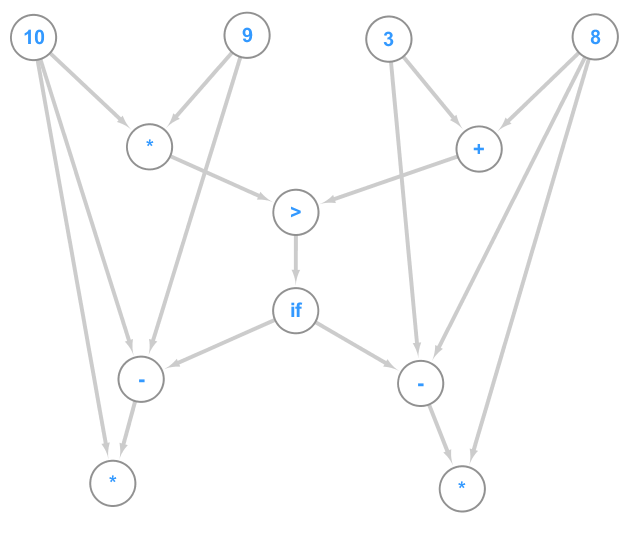
\includegraphics[scale=.7]{figuras/dataflow/pythonCodeDf.png}
    \end{minipage}
    \caption{Exemplo de conversão código para grafo de dependências.
    À esquerda pode ser visto um trecho de código em \emph{python} ao passo que à direita é exibido o grafo dataflow associado.}
    \label{fig:dataflowExemploPython}
\end{figure}

% \subsection{Sucuri} \label{sect:sucuri}

Sucuri \cite{sucuri-original} is a minimalistic Dataflow library for Python language that allows programmers to naturally exploit parallelism through dataflow execution on Von Neumann machines. Sucuri allows transparent execution on computer cluster, relying on Python mechanisms for object serialization (\emph{Pickle}).

Conceptually, a dataflow graph is comprised of nodes that represent tasks, which can be fine-grained (as instructions) or coarse-grained (as functions). Edges connecting nodes represent data-dependencies, meaning a source node will produce a result that will be used by the destination node. When a certain node receives all necessary inputs though its incident edges, it can be dispatched to execution.

Figure \ref{fig:arch} shows Sucuri's structure, where it is possible to observe three main components: \texttt{Graph}, \texttt{Scheduler} and \texttt{Worker}. 

The \texttt{Graph} is just a container object for nodes that represent a dataflow application, each containing:
\begin{itemize}
    \item The list of inputs received so far. When all necessary operands are receive a \emph{matching} occurs and node execution will be triggered.
    \item The function (computation) that should be executed when matching happens for that node.
    \item A list of destination nodes that should receive the result produced.
    \item Specific attributes, such as an unique id that can be used for assigning work to a set of nodes (like in a fork-join approach).
\end{itemize}

When used in a cluster of computers, each of the aforementioned components is replicated in each machine of the cluster, except for the Scheduler, meaning Sucuri adopts a centralized pool of tasks. In \cite{sucuri-distribuida} Sucuri authors implement and evaluate a distributed scheduler for Sucuri, but this version is not employed in this work.

\begin{figure}[htbp]
    \centering
    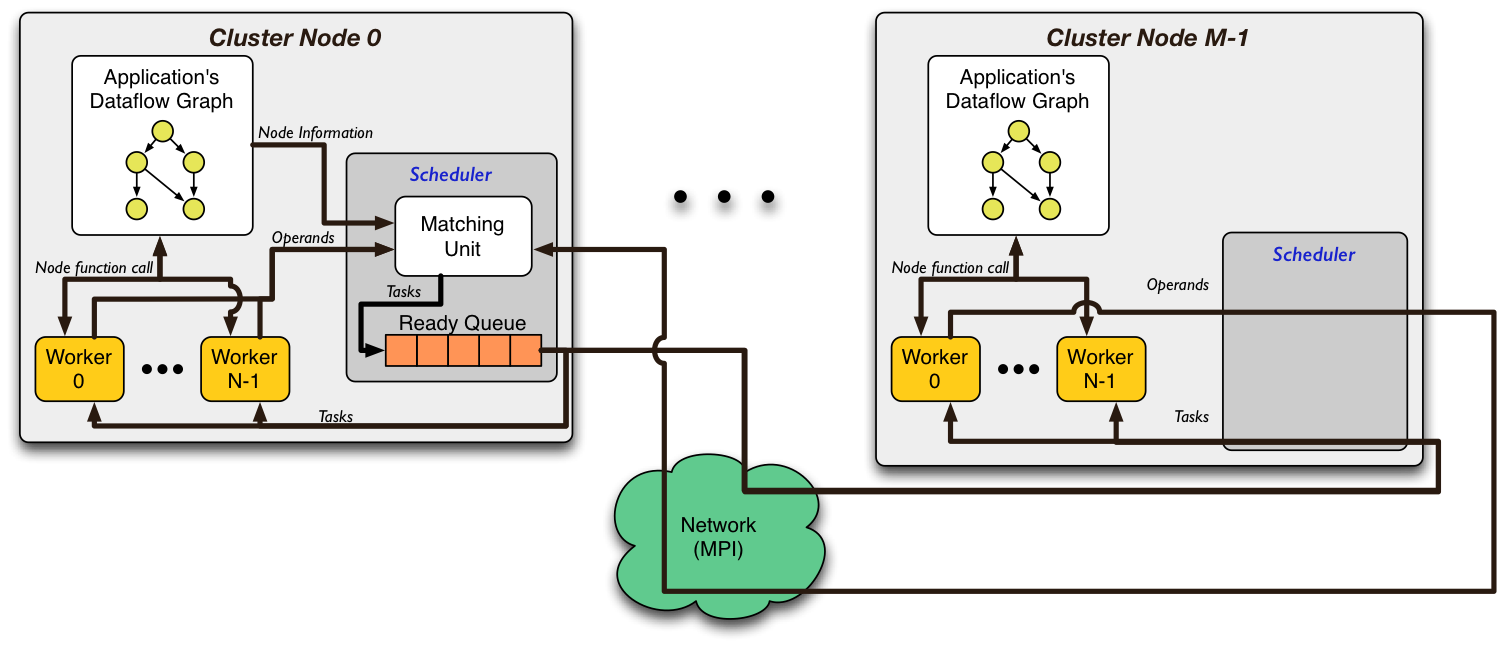
\includegraphics[scale=0.65]{figuras/dataflow/SucuriArchitectureHorizonal.png}
    \caption{The Sucuri Architecture (from \cite{sucuri-original}). The same structure is replicated in each node but only the Scheduler from Cluster Node 0 contains the Matching Unit and the Ready Queue. It is responsible for receiving operands from local Workers and from the others Schedulers and also to generate tasks and put them into the Ready Queue.}
    \label{fig:arch}
\end{figure}

The main \texttt{Scheduler}, placed at Cluster Node 0, is composed of a Matching Unit, a Ready Queue and a Waiting Queue. It is responsible for delivering all operands to the operand list of its destination Node in the Graph. If a match happens, a task is created and put in the Ready Queue. When workers are idle they will request tasks to the \texttt{Scheduler}, that would be fetched from the Ready Queue. The \texttt{Scheduler} placed in the other cluster nodes are more simple and only forwards tasks from the main \texttt{Scheduler} to their local workers and operands from their workers to the main \texttt{Scheduler}. The graph is replicated in all nodes of the Cluster but only the graph in node 0 can receive operands from the main \texttt{Scheduler}.

All communication intra-node between the main components cited above is done via shared memory and between Schedulers from different nodes is done via interface.

Each node of a Sucuri graph is associated with a function that can be implemented by programmers and pass them to node instantiation when creating the dataflow graph. After instantiating the nodes, the programmer can then proceed to connect them using the \texttt{add\_edge()} method, which basically creates a new dependency in the dataflow graph. When the scheduler dispatches a task for execution in a certain worker, that worker will call the \texttt{run()} method of the node corresponding to that task. In most cases, this \texttt{run()} method will just act as a wrapper that calls the function associated with the node during the construction of the graph and send the values returned by the function call to the main scheduler.

Sucuri also provides a set of special nodes that could help programmers devise applications that follow some parallel patterns. For example, a software pipeline application for Sucuri is presented in Fig.~\ref{fig:pipeline}. Panel $A$ shows a graph representation of this pattern and panel $B$ the Sucuri's code for this operation. Notice how new nodes are creates (lines 11-13), added to the graph (lines 17-19) and how edges connecting the nodes are defined (lines 21 and 22). Also, notice the instantiation of the scheduler (line 6) and how to start the schedule after the dataflow graph is defined (line 23).

Figure \ref{fig:pipeline} also shows how a special node \texttt{Source} receives an \emph{iterable} Python object (for instance, a list or a file descriptor) at instantiation. During program execution, the \texttt{run()} method of the \emph{Source} node will be fired only once, since this node works as a root, i.e., has no input operands from the graph and serves to initiate the computation. The execution of such method, however, will typically last until the contents of the iterable object are exhausted. By default the \texttt{Source} node will loop over the iterable object and produce several outputs (messages) that would trigger the execution of the pipeline multiple times. 

Notice that the last node of the pipeline is a special \texttt{Serializer} node, that is responsible for writing the data to a file. It is possible for the data produced by the \texttt{Source} node to be processed out of order by the second node, since the multiple tasks may be scheduled to different workers. Therefore, it is necessary to reorder the data before writing it to the file, in the \texttt{Serializer} node. For that purpose, the data produced by the \texttt{Source} node must be encapsulated in a \texttt{TaggedValue} object, which contains a \texttt{tag} attribute, indicating its position in the ordered data set. The middle node will also send the filtered data inside of a \texttt{TaggedValue} object, with the same tag of the chunk of data it received. The \texttt{Serializer} node then, upon receiving data from the filter node, will store it in a buffer sorted according to the tag. If the tag of the last piece of data received corresponds to the next data to be written to the file, the \texttt{Serializer} node proceeds to pop data from the sorted buffer and write to the file until there is a gap in the ordering, i.e. the chunk of data that is the next to be written has not arrived yet. If the data received by the \texttt{Serializer} is out of order, the node just stores it in the sorted buffer and waits for more data. The \texttt{pin\(\)} method is used to pin the node to a certain worker, which will make it only be executed by that worker. In the case of the example, we pin the nodes that performs I\/O operations on disk to the workers that have direct access to that disk. 

\begin{figure}[htbp]
    \centering
    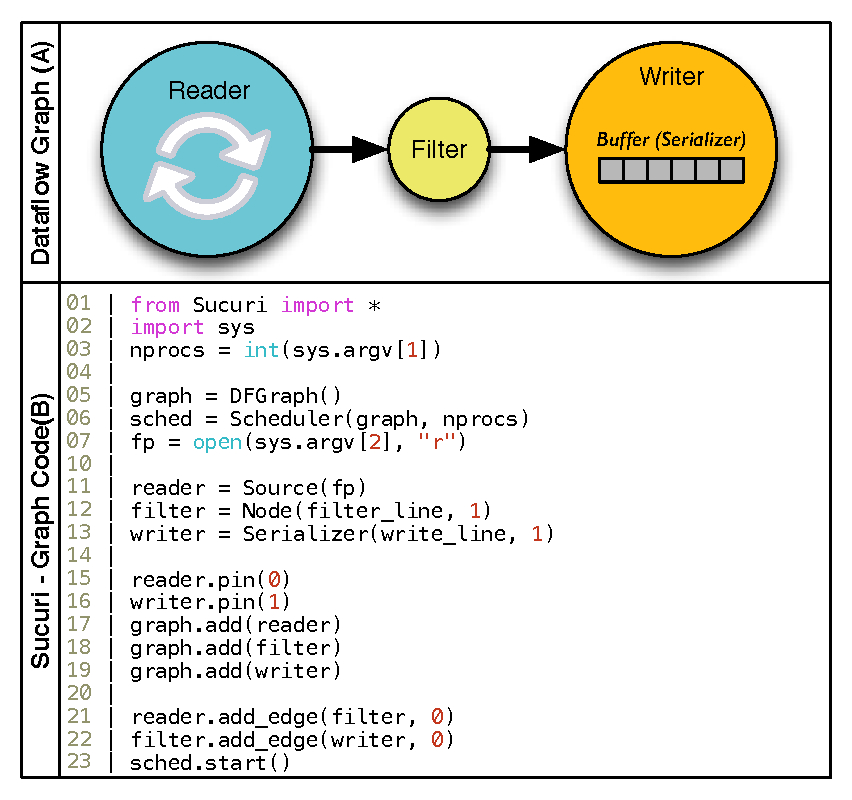
\includegraphics[scale=0.75]{figuras/dataflow/pipeline.eps} 
    \caption{Pipelining with Sucuri. 
    %The data is read from the disk by \texttt{Reader} node encapsulated in a \texttt{TaggedValue} object while a filter is applied by \texttt{Filer} node in a data read previously. As the \texttt{Filter} finish, the \texttt{Writer} node receives and store them in buffer sorted according to the tag. If the tag of the last piece of data received corresponds to the next data to be written to the file, the \texttt{Writer} node proceeds to pop data from the sorted buffer and write to the file.
    Panel $A$ shows the dataflow graph of the application, panel $B$ describes the graph using Sucuri.}
    \label{fig:pipeline}
\end{figure}

One interesting modeling feature that we explore in this paper consists in exploring coarse-grained programming in Sucuri together with fine-grained computing on GPU. This results in a heterogeneous Dataflow/Von Neumann computing, with dataflow nodes performing high performance GPU computing.
This strategy provides greater flexibility for the design of novel algorithms, with greater simplicity than adopting a single computing paradigm (dataflow or von Neumann).



\section{RVND}

O RVND, conforme descrito na Seção~\ref{sec:rvndClassico}, pode ser implementado num grafo dataflow conforme a Figura~\ref{fig:rvndGraph}, onde o nó inicial (\textit{ini}) envia a solução inicial para o primeiro operador de vizinhança (\textit{Swap}), cada nó operador de vizinhança explora todos os movimentos e escolhe o melhor, se este melhora a solução atual então a solução melhorada é enviada para o primeiro né operador (\textit{oper0}) caso contrário a solução é enviada para o próximo nó de enumeração de vizinhança.

\begin{figure}[htbp]
    \centerline{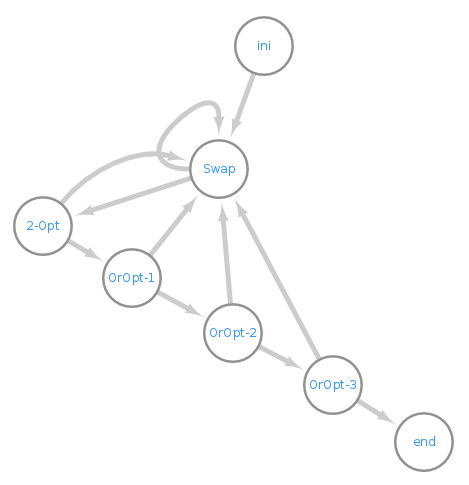
\includegraphics[scale=0.5]{figuras/rvnd/RVND_dataflow_nomes.png}}
    \caption{Arquitetura simplificada do dataflow para o RVND com as vizinhanças utilizadas.}
    \label{fig:rvndGraph}
\end{figure}

A implementação do nó operador (\textit{Swap, 2-Opt, OrOpt-1, OrOpt-2, OrOpt-3}) é tão simples quanto o Algoritmo~\ref{alg:rvndOper} e cada estratégia de vizinhança é atrelada a um nó operador, sendo que a ordem desses é variada para cada execução do método para caracterizar o RVND, a decisão de para qual nó enviar o resultado é tomada pela configuração do dataflow.
Quando a solução atinge o nó final (\textit{end}) esta é salva e o processo termina.

\begin{algorithm}[htpb]
\caption{Nó de vizinhança do RVND}
\label{alg:rvndOper}
\begin{algorithmic}[1]
    \Function{RVND\_Oper}{Solução: $s$}
        \Let{$s'$}{melhor solução de $N^k(s)$}
        \Let{$improvFlag$}{$f(s') < f(s)$}
        \Return{$(s', improvFlag)$}
    \EndFunction
\end{algorithmic}
\end{algorithm}

Pode ser visto destacado na Figura~\ref{fig:rvndGraphDestacado} uma vizinhança com suas ligações ao grafo dataflow, uma de entrada de dados e duas outras de saída que são para o caso de haver ou não uma melhoria no valor da solução.
Para acoplar uma nova vizinhança ao algoritmo basta que seja inserido um novo nó de enumeração com sua entrada de dados vindo do nó anterior e duas saídas de dados, uma retornando para a primeira vizinhança e outra para a vizinhança seguinte, conforme destacado na mesma figura.

\begin{figure}[htbp]
    \centerline{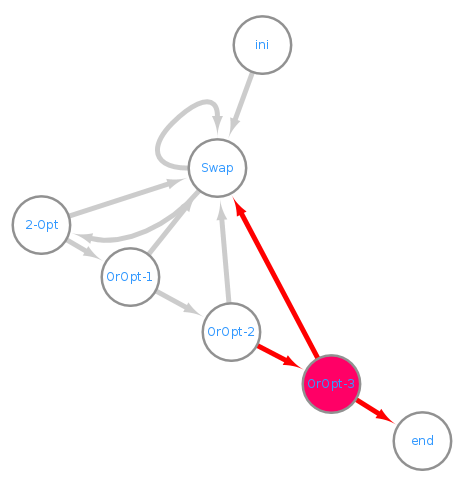
\includegraphics[scale=0.5]{figuras/rvnd/RVND_dataflow_nomesDestacado.png}}
    \caption{Uma vizinhança e suas ligações ao grafo dataflow no RVND.}
    \label{fig:rvndGraphDestacado}
\end{figure}

\subsubsection{Passo iterativo}

Utilizando o termo convencionado na seção~\ref{subsec:passoIterativo}, cada passo iterativo do RVND retorna a melhor solução encontrada para a vizinhança atual.
Assim sendo $N^k$ a vizinhança atual temos o passo iterativo para o RVND expresso na Equação~\ref{eq:rvndPassoIterativo}.
\begin{equation} \label{eq:rvndPassoIterativo}
    \rho^{RVND}(s) = s' \in N^k \quad \textrm{sendo} \quad f(s') < f(s''), \forall s'' \in N^k(s) \land s'' \ne s
\end{equation}
Fazendo uso da notação de movimentos temos podemos escrever \ref{eq:rvndPassoIterativo} como a Equação~\ref{eq:rvndPassoIterativoMovimento}.
\begin{equation} \label{eq:rvndPassoIterativoMovimento}
    \rho^{RVND}(s) = m \circ s \quad \textrm{com} \quad m \in M^k \land \widehat{m} < \widehat{m_i} \mid \forall m_i \in M^k
\end{equation}


\section{DVND} \label{sec:dvndClassico}

O \textit{Distributed Variable Neighborhood Descent} DVND concebido por~\cite{RIOS201839} utiliza múltiplas vizinhanças conforme o faz o VND (\textit{Variable Neighborhood Descent} proposto por \cite{mladenovic1997}) contudo propõe o processamento das vizinhanças de forma distribuída.
Este processamento distribuído se dá pelo escalonamento das tarefas de enumeração das vizinhanças o que naturalmente proporciona a aleatoriedade proposta no RVND.

A implementação em dataflow não pode alcançar uma grande melhoria do RVND em termos de tempo ou qualidade da solução pois o grafo se assemelha a uma cascata (veja a Figura~\ref{fig:rvndGraph}) o que não permite alcançar paralelismo, então se torna natural o uso do método DVND conforme o Algoritmo~\ref{alg:dvnd}. 
A ideia do DVND é que quando uma solução atinge um ótimo local para uma estrutura de vizinhança ainda pode existir um vizinho com melhor valor de função objetivo em uma estrutura de vizinhança diferente, destarte não necessariamente sendo um ótimo local para todas as vizinhanças
Se uma melhoria é encontrada o processo de busca é reiniciado para todas as estratégias de vizinhança.

\begin{algorithm}[htpb]
\caption{DVND clássico}\label{alg:dvnd}
\begin{algorithmic}[1]
    \Function{DVND}{Solução: $s$, Vizinhanças: $N$}
        \Let{$W$}{$\emptyset$}
        \Let{$H$}{$\emptyset$}
        \ForAll{$N_k \in N$}
            \Let{$s_k$}{$s$} \Comment{Solução atual para vizinhança $k$}
            \Let{$H_{k,s}$}{$true$} \Comment{Solução já foi enumerada pela vizinhança}
            \Let{$W_k$}{$false$} \Comment{Vizinhança aguardando solução}
            \State Chame de forma assíncrona $N^k(s_k)$
        \EndFor
        
        \While{$\exists w \in W \mid w = false$}
            \Let{$k$}{join $N^k(s_k)$} \Comment{Aguarda a resposta da vizinhança $N^k$}
            \Let{$s_k$}{Melhor solução de $N^k(s_k)$}
            \If{$f(s_k) < f(s)$}
                \Let{$s$}{$s_k$}
            \EndIf
            
            \Let{$W_k$}{$true$}
            \ForAll{$N_k \in N$}
                \If{$W_k \land \neg H_{k,s}$}
                    \Let{$s_k$}{$s$}
                    \Let{$H_{k,s}$}{$true$}
                    \Let{$W_k$}{$false$}
                    
                    \State Chame de forma assíncrona $N^k(s_k)$
                \EndIf
            \EndFor
        \EndWhile
        \Return{$s$}
    \EndFunction
\end{algorithmic}
\end{algorithm}

Considerando $ \mathcal{M} = M^{DVND} = M^1 \cup M^2 \cup \dots \cup M^k $ o conjunto com os movimentos de todas as vizinhanças usadas pelo DVND, então em termos de movimento temos que a solução $s''$ retornada a cada iteração do DVND pode ser escrita como $s'' = m_z \circ s$ com $m_z \in \mathcal{M}$ e $\widehat{m_z}(s) < \widehat{m_i}(s) \mid \forall m_i \in \mathcal{M}$.
Vale ressaltar que $\mathcal{M} = M^{DVND} = M^{RVND}$, a diferença dos métodos é que a cada iteração o RVND move para a melhor solução da vizinhança atual e no caso do DVND este move para a melhor solução entre todas as vizinhanças.

% Igor, o que acha dessa afirmação?
Numa análise em mais alto nível do RVND (Algoritmo~\ref{alg:rvnd}) e DVND (Algoritmo~\ref{alg:dvnd}), pensando-se à luz das estratégias de \textit{First improvement} e \textit{Best improvement}, o RVND enumera as soluções vizinhas da solução atual vizinhança por vizinhança até encontrar uma solução que a melhore e então retorna para a primeira vizinhança ao passo que o DVND enumera todas as vizinhanças para então optar pela solução de melhor valor.
Desta forma o RVND é uma estratégia de \textit{first improvement} no contexto de vizinhanças de solução e o DVND uma estratégia de \textit{best improvement}.

